% !TeX encoding = utf-8
% !TEX spellcheck = en-us
% !TeX program = xelatex

\documentclass[english]{lightweightbook}

\booktitle{Lightweight Book Theme Demo}
\booksubtitle{A practical guide to the Lightweight Book class}
\bookauthor{Ruiyang Zhou}
\bookpublisher{Creation Theme Collection}
\bookedition{2026 Revision}
\bookdate{March 13, 2026}
\booktagline{Build modern books and reports with a clean, reusable interface.}

\begin{document}
    \frontmatter
    \maketitle

    \begin{bookabstract}
        This document is the official demo for the Lightweight Book theme.
        This demo introduces the design goals, command interface, document structure,
        and common writing components with runnable examples.
    \end{bookabstract}

    \begin{preface}
        If you are new to this theme, read this file from top to bottom once,
        then reuse the code blocks as a starter template. The class already bundles
        heading style, color system, theorem setup, callout boxes, and front-matter pages.
    \end{preface}

    \printbookcontents

    \mainmatter


    \chapter{Theme Overview}
    \begin{chapterquote}[Lightweight Book provides a modern class for books and reports.]
        The original section-style experiment has evolved into a full class.
        It now controls the cover, typography, chapter and section hierarchy,
        theorem blocks, utility callouts, and metadata output in a single interface.
    \end{chapterquote}


    \section{What this theme gives you}
    Lightweight Book is designed for notes, technical reports, and compact books.
    It reduces repeated preamble code and keeps visual style consistent across files.

    \begin{summarybox}
        Lightweight Book offers a clean writing experience with modern defaults and reusable components.
    \end{summarybox}

    \begin{table}[htbp]
        \centering
        \caption{Core capabilities of Lightweight Book}
        \begin{tabularx}{\textwidth}{@{}>{\raggedright\arraybackslash}p{0.30\textwidth}>{\raggedright\arraybackslash}X@{}}
            \toprule
            Capability & What it does \\
            \midrule
            Cover metadata commands & Generates a modern title page and fills PDF metadata fields. \\
            Front-matter environments & Adds abstract, preface, acknowledgements, and dedication pages with TOC support. \\
            Section and chapter style & Applies a consistent heading hierarchy and visual identity. \\
            Math and theorem setup & Provides theorem-like environments with chapter-based numbering. \\
            Callout and code blocks & Includes reusable summary, tip, warning, example, and listing styles. \\
            \bottomrule
        \end{tabularx}
    \end{table}


    \section{Compile requirements}
    \begin{tipbox}
        Compile with \texttt{XeLaTeX}. The class depends on \texttt{fontspec} and \texttt{ctexbook}.
    \end{tipbox}

    \begin{warningbox}
        Keep the \texttt{fonts/} folder beside \texttt{lightweightbook.cls} unless you customize font paths.
    \end{warningbox}


    \chapter{How to Start a New Document}


    \section{Minimal template}
    Copy the snippet below into a new \texttt{.tex} file to start quickly.

    \begin{codeblock}[language={[LaTeX]TeX},caption={Minimal Lightweight Book template},label={lst:minimal-template}]
        \documentclass[english]{lightweightbook}

        \booktitle{My Lightweight Book Notes}
        \booksubtitle{Optional subtitle}
        \bookauthor{Author Name}
        \bookpublisher{Organization}
        \bookedition{v1.0}
        \bookdate{March 2026}
        \booktagline{Optional short description}

        \begin{document}
            \frontmatter
            \maketitle
            \printbookcontents

            \mainmatter


            \chapter{Introduction}
            Your content starts here.

            \backmatter
        \end{document}
    \end{codeblock}


    \section{Metadata command reference}
    \begin{table}[htbp]
        \centering
        \caption{Cover and metadata commands}
        \begin{tabularx}{\textwidth}{@{}>{\raggedright\arraybackslash}p{0.32\textwidth}>{\raggedright\arraybackslash}X@{}}
            \toprule
            Command & Description \\
            \midrule
            \texttt{\textbackslash booktitle\{...\}} & Main title shown on cover and used in PDF title metadata. \\
            \texttt{\textbackslash booksubtitle\{...\}} & Optional subtitle on cover. \\
            \texttt{\textbackslash bookauthor\{...\}} & Author line on cover and PDF author metadata. \\
            \texttt{\textbackslash bookpublisher\{...\}} & Publisher or affiliation text block. \\
            \texttt{\textbackslash bookedition\{...\}} & Optional edition or release label. \\
            \texttt{\textbackslash bookdate\{...\}} & Date text on cover. \\
            \texttt{\textbackslash booktagline\{...\}} & Short theme or subject line; also used for PDF subject metadata. \\
            \texttt{\textbackslash bookcoverimage\{...\}} & Optional image path for cover artwork overlay. \\
            \bottomrule
        \end{tabularx}
    \end{table}


    \chapter{Detailed Feature Demonstration}


    \section{Front matter helpers}
    The class includes dedicated environments for common publishing sections.
    In a real project, these typically appear in front matter or back matter.

    \begin{codeblock}[language={[LaTeX]TeX},caption={Front matter and back matter helpers}]
        \begin{bookabstract}
            Brief project summary.
        \end{bookabstract}

        \begin{preface}
            Context, audience, and scope.
        \end{preface}

        \begin{acknowledgements}
            Credits and thanks.
        \end{acknowledgements}
    \end{codeblock}


    \section{Theorem environments}
    \begin{definition}
        A reusable document class is a stable interface that separates content from presentation.
    \end{definition}

    \begin{theorem}
        Centralizing layout in one class file improves consistency and lowers maintenance cost.
    \end{theorem}

    \begin{proof}
        When style commands are declared once in the class, documents avoid duplicated preambles.
        Future visual changes are made in one location and propagate to all documents.
    \end{proof}

    \begin{examplebox}
        Use \texttt{theorem}, \texttt{lemma}, \texttt{proposition}, \texttt{corollary},
        \texttt{definition}, \texttt{example}, and \texttt{remark} directly.
    \end{examplebox}


    \section{Callout boxes}
    \begin{summarybox}
        \texttt{summarybox} is ideal for key takeaways at the end of a section.
    \end{summarybox}

    \begin{tipbox}
        \texttt{tipbox} works well for writing and formatting guidance.
    \end{tipbox}

    \begin{warningbox}
        \texttt{warningbox} highlights constraints and migration notes.
    \end{warningbox}


    \section{Figure and graphics style}
    The class already loads TikZ, so diagrams can be added directly.

    \begin{figure}[htbp]
        \centering
        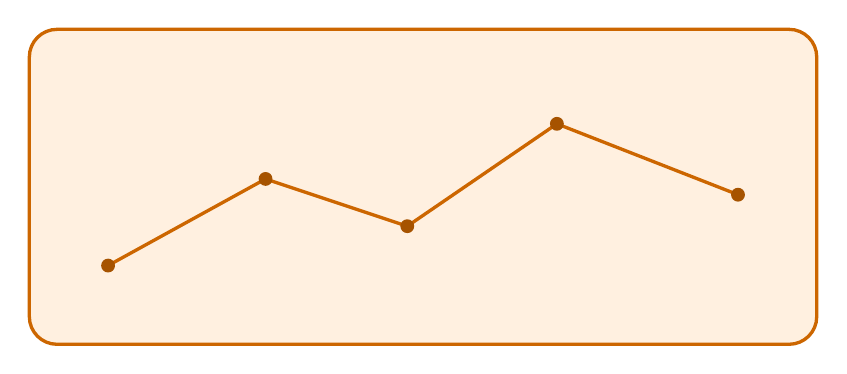
\begin{tikzpicture}[x=1cm,y=1cm]
            \fill[orange!12,rounded corners=10pt] (0,0) rectangle (10,4);
            \draw[orange!80!black,line width=1.2pt,rounded corners=10pt] (0,0) rectangle (10,4);
            \draw[orange!80!black,line width=1.2pt] (1,1) -- (3.0,2.1) -- (4.8,1.5) -- (6.7,2.8) -- (9.0,1.9);
            \foreach \x/\y in {1/1,3.0/2.1,4.8/1.5,6.7/2.8,9.0/1.9}{
                \fill[orange!65!black] (\x,\y) circle (2.5pt);
            }
        \end{tikzpicture}
        \caption{Sample inline chart styled with class color variables}
    \end{figure}


    \chapter{Recommended Project Layout}


    \section{Suggested file organization}
    For larger projects, keep content modular.

    \begin{codeblock}[language={[LaTeX]TeX},caption={Example project split}]
        project/
        |- lightweightbook.cls
        |- fonts/
        |- main.tex
        |- chapters/
        |  |- 01-introduction.tex
        |  |- 02-methods.tex
        |  |- 03-results.tex
        |- figures/
        |- references.bib
    \end{codeblock}

    \backmatter
    \begin{acknowledgements}
        This demo serves as both a showcase and a usage reference for Lightweight Book.
        Keep it as a baseline when adding new components to the class.
    \end{acknowledgements}

\end{document}
